\documentclass{standalone}
\usepackage{tikz}

\usetikzlibrary{matrix,positioning,fit}
\usepackage[export]{adjustbox}
\usepackage{tcolorbox}


	
\def\layersep{2.5cm}
%\pagestyle{empty}

\begin{document}
	
	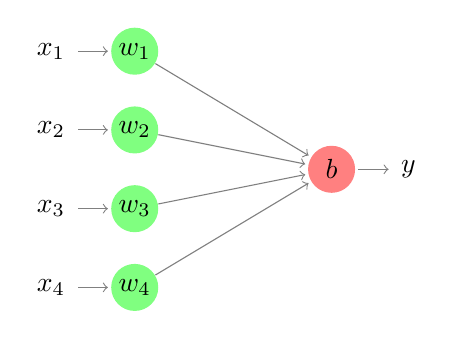
\begin{tikzpicture}[shorten >=1pt,->,draw=black!50, node distance=\layersep]
	\tikzstyle{every pin edge}=[<-,shorten <=1pt]
	\tikzstyle{neuron}=[circle,fill=black!25,minimum size=17pt,inner sep=0pt]
	\tikzstyle{input neuron}=[neuron, fill=green!50];
	\tikzstyle{output neuron}=[neuron, fill=red!50];
	\tikzstyle{hidden neuron}=[neuron, fill=blue!50];
	\tikzstyle{annot} = [text width=4em, text centered]
	
	\pgfmathsetmacro{\nIn}{4}
	\pgfmathsetmacro{\nHa}{5}
	\pgfmathsetmacro{\nHb}{7}
	\pgfmathsetmacro{\nHc}{5}
	\pgfmathsetmacro{\nOut}{1}
	
	% Draw the input layer nodes
	\foreach \name / \y in {1,...,\nIn}
	% This is the same as writing \foreach \name / \y in {1/1,2/2,3/3,4/4}
	\node[input neuron, pin=left:$x_\y$] (I-\name) at (0,-\y) {$w_\y$};
	
	% Draw the hidden layer nodes

	% Draw the output layer node
	\foreach \name / \y in {1,...,\nOut}
	\path[yshift=-1.5cm]
	node[output neuron, pin={[pin edge={->}]right:$y$}, right of=NodeHb] (O-\name) at (0em,-\y cm) {$b$};
%	\node[output neuron,pin={[pin edge={->}]right:y}, right of=H2-3] (O) {};
	
	% Connect every node in the input layer with every node in the
	% hidden layer.
	
	\foreach \source in {1,...,\nIn}
	\foreach \dest in {1,...,\nOut}
	\path (I-\source) edge (O-\dest);
	
	

	\end{tikzpicture}
	
	
\end{document}